% coding:utf-8

%----------------------------------------
%FOSAMATH, a LaTeX-Code for a mathematical summary for basic analysis
%Copyright (C) 2013, Daniel Winz, Ervin Mazlagic, Adrian Imboden, Philipp Langer

%This program is free software; you can redistribute it and/or
%modify it under the terms of the GNU General Public License
%as published by the Free Software Foundation; either version 2
%of the License, or (at your option) any later version.

%This program is distributed in the hope that it will be useful,
%but WITHOUT ANY WARRANTY; without even the implied warranty of
%MERCHANTABILITY or FITNESS FOR A PARTICULAR PURPOSE.  See the
%GNU General Public License for more details.
%----------------------------------------

% coding:utf-8
\section{Definition Differentialgleichungen}
Gleichungen, in der eine Variable, eine von dieser Variable abhängige Funktion 
und Ableitungen beliebigen Grades dieser Funktion vorkommen, werden 
Differentialgleichungen genannt. 
\[ F(x, y, y', y'', \ldots, y^{(n)})=0 \]
$x$ heisst dabei unabhängige und $y$ abhängige Variable. Dafür können auch 
andere Buchstaben als $x$ und $y$ verwendet werden. 
Ableitungen nach t werden auch als $\dot{y}$ geschrieben. 

\section{Grundbegriffe}

\subsection{Ordnung}
Die Ordnung einer Differentialgleichung wird durch die höchste vorkommende 
Ordnung der Ableitungen von $y$ bestimmt. 

\subsection{Grad}
Der Grad einer Differentialgleichung wird durch die höchste vorkommende Potenz 
von $y$ oder den Ableitungen von $y$ bestimmt. Potenzen der unabhängigen 
Variable werden dabei nicht berücksichtigt. 
\subsubsection*{Achtung:}
$y \cdot y' \quad \rightarrow \quad$ Grad 2

\subsubsection{Grad 1}
Differentialgleichungen vom Grad 1 nennt man linear. 

\subsection{Lösungen}
Eine Gleichung der Form
\[ F(x, y, y', y'', \ldots, y^{(n)})=0 \]
besitzt eine allgemeine Lösung. Diese enthält $n$ Parameter ($n$-parametrige 
Kurvenschar). Jede Kombination dieser Parameter ergibt eine spezielle bzw. 
partikuläre Lösung. Durch das Festlegen spezieller Werte für 
$y, y', y'', \ldots, y^{(n)}$ an einer beliebigen Stelle $x_0$ erhält man Werte 
für die $n$ Parameter und somit eine partikuläre Lösung. 

\section{Richtungsfeld und Trajektorien}
Ein Richtungsfeld ist ein Abbild einer Differentialgleichung im Raum.
Dabei wird jedem Punkt im Raum eine Steigung (\emph{Differential})
zugewiesen. Im folgenden ein Beispiel eines solchen Richtungsfeldes.

\begin{figure}[h!]
	\centering
	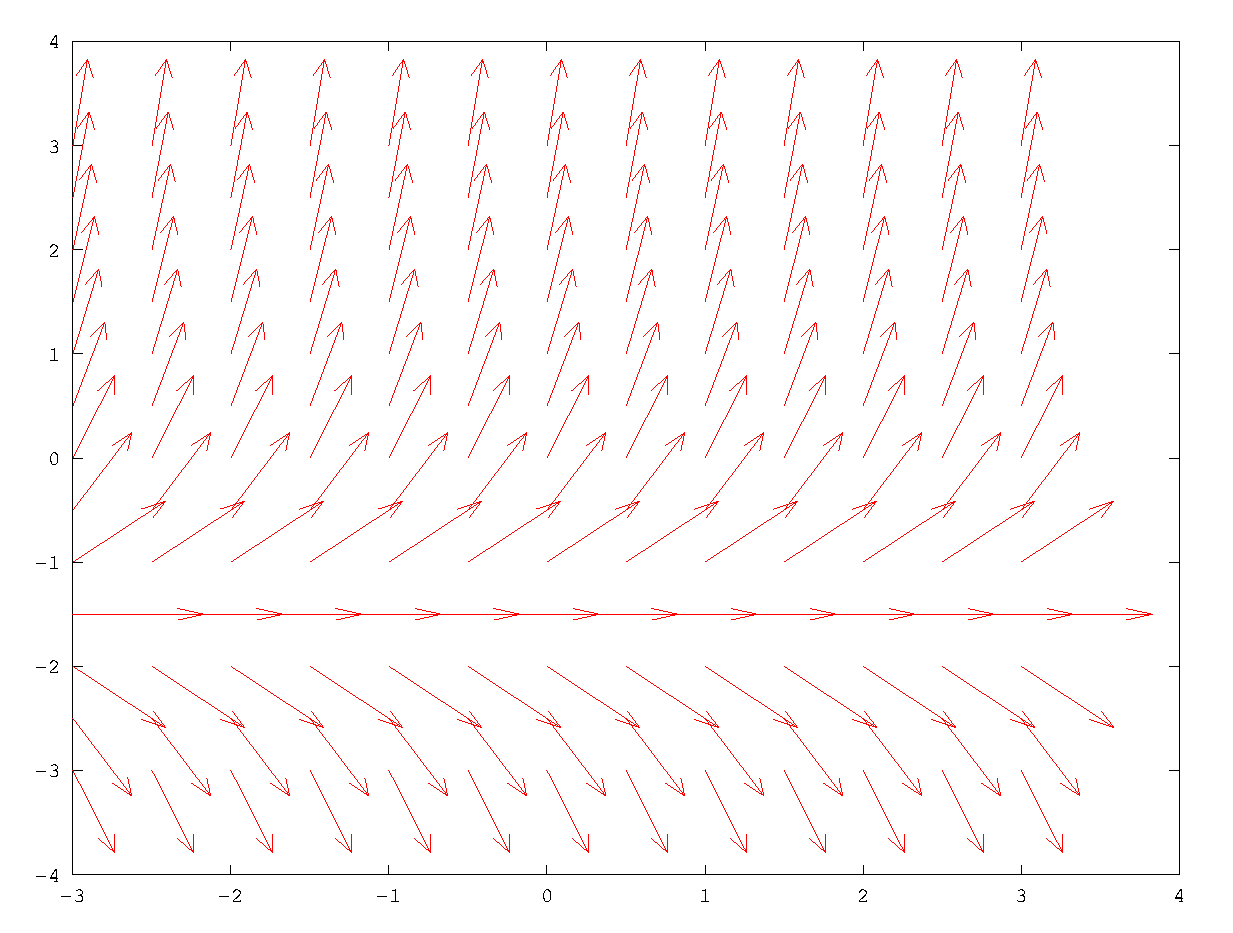
\includegraphics[width=0.8\textwidth]{field.eps}
	\caption{Richtungsfeld der Differentialgleichung $y'=3+2y$}
\end{figure}

\noindent
Die Berechnung der einzelnen Punkte erfolgt durch reines einsetzen.
Z.B. für den Punkt $P(x=1, y=-1)$ ergibt sich $3+2(-1)=1$ usw.

\subsection{Trajektorien}
Trajektorien sind Bahnkurven die die Lösung einer Differentialgleichung
darstellen. Es handelt sich dabei um eine Kurvenschar, welche eine andere
Kurvenschar mit immer dem selben Winkel schneidet. Wenn dieser Winkel
$90^{\circ}$ beträgt, so nennt man diese othogonale trajektorie.
Um eine solche orthogonale Trajektorie zu berechnen kann in drei Schritten
vorgegangen werden.
\begin{enumerate}
  \item Differentialgleichung der Kurvenschar aufstellen in der Form
	$y'=g(x,y)$
  \item Differentialgleichung der orthogonalen Trajektorien bilden
	mit Hilfe der Regel, dass $m_2=-\frac{1}{m_1}$ für orthogonale
	Kurven ist. Somit ergibt sich $y'=-\frac{1}{g(x,y)}$
  \item Allgemeine Lösung der im zweiten Schritt erstellten
	Differentialgleichung finden (z.B. mit \emph{Trennung der Variablen}
	oder \emph{Variation der Konstanten}). Diese Lösung ist dann die 
	eigentliche Trajektorie.
\end{enumerate}

\section{Lösungsverfahren}

\subsection{Variation der Konstanten \\(Lineare Gleichung 1. Ordnung)}
\begin{enumerate}
  \item Inhomogene Gleichung notieren / aufstellen (I)
  \item Normalform bilden / aufstellen (N)
  \item Homogene Gleichung bilden / aufstellen (H)
  \item $g(x)$ und $G(x)$ bestimmen ($G(x) = \int g(x)$)
  \item $G(x)$ einsetzen in die allgemeine Lösung $y_h=c \cdot e^{-G(x)}$
        $\rightarrow$ so erhält man die allgemeine Lösung der 
        homogenen Gleichung (H)
  \item Variation der Konstanten d.h. aus dem c wird eine Funktion $K(x)$ 
        $(\rightarrow y= \ldots)$
  \item Funktion ableiten (für $y'$)
  \item Die neuen Definitionen für $y$ und $y'$ einsetzen in die Normalform (N) 
  \item Auflösen nach $K(x)$ (durch Integration)
  \item Einsetzen in die allgemeine Lösung der homogenen Gleichung ($y_h$)
\end{enumerate}
